% ----------------------------------------------------------
\chapter{Desenvolvimento da Técnica}\label{cap:desenvolvimento}

Durante esse capítulo serão detalhadas as técnicas e passos utilizados para atingir os objetivos citados no Capítulo 1, iniciando com o desenvolvimento de ferramentas de apoio, experimentos com a aplicação de métodos esteganográficos existentes na ISA do RISC-V e a execução do projeto em uma aplicação de linha de comando de uso geral.

Ao longo deste capítulo serão introduzidos conceitos necessários para a compreensão do algoritmo proposto como objetivo, com uma pesquisa calcada tanto em materiais e documentos históricos quanto produções acadêmicas recentes de maior relevância.

\subsection{Aplicações para Experimentos e Validações}

Para avaliar os resultados obtidos pelas técnicas de esteganografia e validar o ferramental de apoio desenvolvido durante este trabalho foram utilizado dois conjuntos de classes distintas de programas como objetos de experimento. O primeiro conjunto contém a compilação de 2 sistemas operacionais, o segundo conjunto é composto 22 programas utilitários de bancos de dados. Os sistemas operacionais foram selecionados devido a alta gama de operações distintas realizadas por esse tipo de programa durante sua execução. Os utilitários com enfoque para bancos de dados foram escolhidos por possuirem em seu código algoritmos variados de ordenação, busca e transformação de dados, com o intuito de entender se um programa altamente focado em operações em disco é mais suscetível a técnicas de esteganografia. 

Para ambos os conjuntos de programas foi utilizado o processo de compilação cruzada a partir de uma máquina x86 tendo como arquitetura alvo o RISC-V para eliminar a necessidade de possuir uma placa física implementando RISC-V. No primeiro conjunto os softwares utilizados foram o EPOS (Embedded Parallel Operating System), desenvolvido com o propósito de ser um SO enxuto e eficiente capaz de ser executado em microprocessadores de sistemas embarcados e o Linux, um SO de propósito geral utilizado na maioria dos dispositivos pelo mundo e que conta com funcionalidades mais variadas e robustas do que o primeiro. Para o segundo conjunto foram utilizados os utilitários gerados na compilação do SGBD PostgreSQL, que incluem o próprio SGBD e outros módulos utilizados para funcionalidades específicas do software. As Tabelas \ref{tab:prog_1} e \ref{tab:prog_2} contém os nomes, versões e tamanhos de arquivos (descritos em bits) de todos os softwares utilizados para os experimentos, separados em seus conjuntos. 

\begin{table}[htb]
    \centering
    
    \begin{tabular}{|c|c|c|}
        \hline
        Programa & Versão  & Tamanho\\
        \hline
        Linux & v6.5 & 150792320 \\
        \hline
        EPOS & v2.2.2 & 288128 \\
        \hline
    \end{tabular}
    \caption{Conjunto 1 de programas utilizados nos experimentos}
    \label{tab:prog_1}
\end{table}

\begin{table}[htb]
    \centering
    
    \begin{tabular}{|c|c|c|}
        \hline
        Programa & Versão  & Tamanho\\
        \hline
        initdb & v16.0.0 & 1252608 \\
        \hline
        pgbench & v16.0.0 & 1502784 \\
        \hline
        pg\_amcheck & v16.0.0 & 809536 \\
        \hline
        pg\_archivecleanup & v16.0.0 & 372736 \\
        \hline
        pg\_basebackup & v16.0.0 & 1197632 \\
        \hline
        pg\_checksums & v16.0.0 & 657152 \\
        \hline
        pg\_config & v16.0.0 & 360512 \\
        \hline
        pg\_controldata & v16.0.0 & 475456 \\
        \hline
        pg\_ctl & v16.0.0 & 566784 \\
        \hline
        pg\_dump & v16.0.0 & 2857344 \\
        \hline
        pg\_dumpall & v16.0.0 & 1003264 \\
        \hline
        pg\_receivewal & v16.0.0 & 876736 \\
        \hline
        pg\_recvlogical & v16.0.0 & 841408 \\
        \hline
        pg\_resetwal & v16.0.0 & 524928 \\
        \hline
        pg\_restore & v16.0.0 & 1414208 \\
        \hline
        pg\_rewind & v16.0.0 & 1252928 \\
        \hline
        pg\_test\_fsync & v16.0.0 & 405504 \\
        \hline
        pg\_test\_timing & v16.0.0 & 331136 \\
        \hline
        pg\_upgrade & v16.0.0 & 1247936 \\
        \hline
        pg\_verifybackup & v16.0.0 & 864768 \\
        \hline
        pg\_waldump & v16.0.0 & 843392 \\
        \hline
        psql & v16.0.0 & 3672768 \\
        \hline
    \end{tabular}
    \caption{Conjunto 2 de programas utilizados nos experimentos}
    \label{tab:prog_2}
\end{table}
\section{Ferramental de Suporte}

A fim de alcançar os objetivos propostos por este trabalho foi necessário estudar tópicos satélites e desenvolver aplicações utilitárias quando não houvessem projetos \texttt{open source} capazes de suprir a necessidade. Essas aplicações estão distribuídas no formato de módulos Python e podem ser usadas de forma independente.

\subsection{\textit{Parser} para arquivos ELF}

A partir da decisão de trabalhar diretamente em arquivos binários modificando sua estrutura e conteúdo base com o intuito de esconder informações se cria a necessidade de poder abrir, interpretar, analisar e editar arquivos no formato de escolha. Como definido no capítulo passado, este trabalho foca em explorar o formato ELF utilizado amplamente em sistemas Unix. Apesar da existência de utilitários capazes de executar essa tarefa a decisão por desenvolver o \textit{parser} dentro projeto foi tomada pela facilidade em analisar apenas as informações estritamente necessárias para encontrar trechos de instruções de máquina dentro do arquivo, otimizando a performance geral do código.

O funcionamento do \textit{parser} é baseado na leitura de cabeçalhos contendo as informações sobre as seções e segmentos de um arquivo ELF, codificados de forma numérica correspondente a tabelas definidas na especificação do formato. Primeiramente fazemos a leitura do \textit{ELF Header} para nos certificarmos de que o arquivo foi compilado para a arquitetura RISC-V e extraímos informações importantes para os próximos passos, como a ordenação dos \textit{bytes}, o número de seções e segmentos e o índice da tabela de símbolos. Para os objetivos da aplicação desenvolvida, os segmentos serão ignoradas pelo algoritmo, utilizando apenas seções para encontrar porções de código.

Em seguida fazemos a leitura sequencial dos cabeçalhos de seções, utilizando os dados sobre permissões e tipo para identificar trechos de código no arquivo. Ao encontrar uma seção de código é possível pular para seu endereço relativo e retornar os blocos de 32 \textit{bits} correspondentes às instruções de máquina contidas no código. Esse passo do algoritmo é realizado até que a seção seja esgotada, ao ponto em que será buscada a próxima seção para que se repitam os passos anteriores até o esgotamento do próprio arquivo. Com esse processo finalizado temos a lista completa de instruções contidas no programa e já é possível manipulá-las.

% TODO: colocar um diagrama do parser

\subsection{Decodificador e Codificador  para instruções RISC-V}

Após a extração completa de todas as instruções presentes em um binário resta apenas uma longa lista de números com 32 \textit{bits} sem um significado claro para um leitor humano. Para que qualquer técnica esteganográfica seja aplicada sobre uma mídia digital é necessário compreender a semântica dos dados, de modo a evitar o corrompimento acidental da informação contida. Com o propósito de decodificar as instruções para um formato mais legível por seres humanos foi desenvolvido um decodificador de instruções capaz de receber um objeto \textit{bytes} e retornar a instrução correspondente escrita em Assembly.

A especificação do RISC-V introduz conjuntos de instruções base e extensões de propósitos específicos com suas próprias instruções que evoluem com o passar das versões da plataforma, obedecendo formatos de codificação de instruções que definem a posição e semântica dos campos dentro dos 32 bits disponíveis. O conjunto base contém 6 formatos definidos capazes de codificar as instruções mais básicas para o funcionamento de um processador RISC-V, esses formatos estão descritos nas especificações técnicas da arquitetura \cite{riscv_manual_vol1}. 

\begin{figure}[!htb]
     \centering
     \caption{Formatos de Instrução disponíveis na ISA base do RISC-V.}
     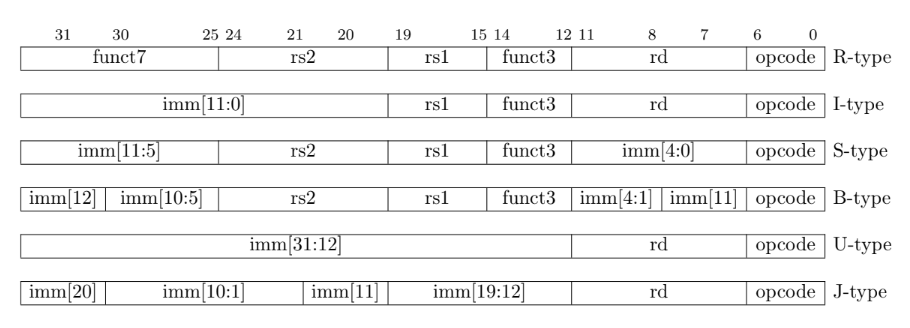
\includegraphics[width=13cm]{images/TCC3.png}
     \legend{Autor: Retirado de \cite{riscv_manual_vol1}}
     \label{}
\end{figure}

Para os propósitos desejados nessa implementação cobrir estes 6 tipos é suficiente, dado que formatos específicos de extensões são menos comuns em programas compilados e podem variar conforme os processadores que adotam a arquitetura. O processo de decodificação foi realizado de forma a identificar inicialmente a qual formato uma instrução pertence utilizando o campo \textit{opcode} que compreende os 7 primeiros bits de cada conjunto de 32 bits gerados pelo compilador. Após a identificação do formato, os demais campos são separados utilizando operações binárias, respeitando particularidades de campos com sinal aritmético para valores numéricos e consultando as tabelas de operações descritas na especificação da ISA. Com todos os campos já traduzidos a instrução é montada em Assembly já com seu mnemônico, registradores e operandos identificados. 

Após a decodificação é criado também um objeto editável contendo os campos de cada instrução para que seja possível alterar os valores representados em alto nível, expondo um método capaz de realizar a transformação reversa, utilizando os campos da instrução para gerar sua contraparte binária. Dessa forma, uma instrução pode ser decodificada, alterada e então recodificada de volta para seu formato binário, podendo ser sobrescrita no arquivo fonte. Esse processo em conjunto com o \textit{parser} de arquivos ELF permite a livre manipulação de qualquer instrução presente em um binário compilado para RISC-V e é a base utilizada posteriormente pelo algoritmo esteganográfico para inserir dados na mídia de destino.

A implementação do decodificador e codificador foi baseada no trabalho de pesquisadores da Universidade de Columbia, desenvolvido na linguagem Javascript com propósitos educacionais \cite{rvcodec}. O projeto \textit{rvcodec.js} visa facilitar o ensino da ISA disponibilizando uma ferramenta online para conversão de instruções e cobre as principais extensões da plataforma além do conjunto base.

\subsubsection{Experimento de Validação}

Os dois conjuntos de testes foram utilizados como método de avaliação da capacidade de decodificação do módulo apresentado, utilizando como métrica a razão entre a quantidade de instruções presentes no programa e a quantidade de instruções que foram decodificadas após o processo. O esperado desse experimento era verificar se os 6 formatos de instrução da ISA base cobrem uma porção suficientemente grande de um binário arbitrário para que seja possível obter taxas de codificação satisfatórias posteriormente. Analisando resultados do experimento presentes nas Tabelas 2 e 3 pode-se notar que a cobertura da ISA base ocupa altas taxas dentro das seções de código do programa, o que indica o potencial para níveis sólidos de codificação de informação apenas com instruções desses formatos.

\begin{table}[!h]
    \centering
    
    \begin{tabular}{|c|c|}
        \hline
        Programa & Percentual de Instruções Decodificadas \\
        \hline
        Linux & 63.55\% \\
        \hline
        EPOS & 70.63\% \\
        \hline
    \end{tabular}
    \caption{Resultados do Experimento do Decodificador para o Conjunto 1}
    \label{tab:exp1_1}
\end{table}

\begin{table}[!h]
    \centering
    
    \begin{tabular}{|c|c|}
        \hline
        Programa & Percentual de Instruções Decodificadas \\
        \hline
        initdb & 76.25\% \\
        \hline
        pgbench & 66.07\% \\
        \hline
        pg\_amcheck & 61.71\% \\
        \hline
        pg\_archivecleanup & 64.58\% \\
        \hline
        pg\_basebackup & 68.58\% \\
        \hline
        pg\_checksums & 63.47\% \\
        \hline
        pg\_config & 67.76\% \\
        \hline
        pg\_controldata & 65.86\% \\
        \hline
        pg\_ctl & 68.65\% \\
        \hline
        pg\_dump & 68.77\% \\
        \hline
        pg\_dumpall & 75.62\% \\
        \hline
        pg\_receivewal & 63.36\% \\
        \hline
        pg\_recvlogical & 64.32\% \\
        \hline
        pg\_resetwal & 65.45\% \\
        \hline
        pg\_restore & 68.59\% \\
        \hline
        pg\_rewind & 66.74\% \\
        \hline
        pg\_test\_fsync & 61.10\% \\
        \hline
        pg\_test\_timing & 65.93\% \\
        \hline
        pg\_upgrade & 76.21\% \\
        \hline
        pg\_verifybackup & 61.90\% \\
        \hline
        pg\_waldump & 63.22\% \\
        \hline
        psql & 69.99\% \\
        \hline
    \end{tabular}
    \caption{Resultados do Experimento do Decodificador para o Conjunto 2}
    \label{tab:exp1_2}
\end{table}

\section{Aplicação de Técnicas Conhecidas}
% ----------------------------------------------------------
Nessa seção está descrito todo o processo, análise e aplicação de técnicas já conhecidas na litetura para codificação de informação em arquivos binários, a fim de verificar sua viabilidade quando transpostas para a arquitetura RISC-V. Foram analisadas apenas técnicas cuja aplicação não envolvem alteração do tamanho do arquivo final ou realocação de endereços ou etiquetas, de forma a manter a viabilidade da implementação para uma gama maior de casos de uso.

\subsection{Alocação de Registradores}

A especificação atual da arquitetura RISC-V prevê 32 registradores de 32 bits para serem utilizados com valores inteiros e outros 32 registradores disponíveis para valores de ponto flutuante, sendo que apenas 8 registradores em cada um desses conjuntos é reservado para alocação de argumentos. Apesar de teoricamente ser possível codificar bits utilizando a escolha dos registradores alocados para cada chamada de função, a convenção de chamadas prevê que esses registradores sejam escolhidos de forma ordenada e crescente, impedindo o uso prático dessa abordagem para implementações \cite{riscv_manual_psabi}.

\subsection{Escalonamento de Instruções}

Certas operações de alto nível quando executadas pelo processador passam por um desmembramento em duas ou mais instruções nativas que podem ser independentes entre si, gerando uma decisão de ordenação que pode ser explorada com o intuito de codificar bits de informação. Tal técnica foi utilizada por Anckaert \textit{et al} (2004) com a arquitetura alvo sendo IA-32, uma arquitetura CISC que dispõe de um número elevado de instruções redundantes ou semelhantes que podem performar operações equivalentes, portanto seus resultados são satisfatórios.

Entretanto, quando o contexto é alterado para uma arquitetura RISC o número de permutações equivalentes a  cada operação de alto nível tende a ser reduzido, impactando na eficiência desse método. Além disso o esforço necessário a ser empregado para essa técnica também é custoso pois requer a implementação de uma ferramenta capaz de gerar todas as permutações possíveis para cada procedimento a que se deseje explorar. A partir do entendimento de que esse método possui um alto custo temporal de implementação e a expectativa de resultados é baixa, o escalonamento de instruções não será abordado durante a execução desse trabalho.

\subsection{Substituição de Instruções Equivalentes}

A estratégia de utilizar escolhas dentro de uma única instrução como estrutura de codificação binária é amplamente utilizada por autores desde os primeiros trabalhos realizados na área, El-Khalil e Keromytis (2004) baseiam sua solução em criar tabelas de instruções equivalentes e atribuir um valor para cada alternativa, dessa forma para cada instrução pertencente a um conjunto de instruções equivalentes, podemos codificar log2(n) bits, sendo n o tamanho do conjunto. Os autores catalogaram 18 conjuntos de equivalência dentro da ISA \texttt{x86}, variando entre operações aritméticas e binárias, com equivalências produzidas por ordem de operandos e inversas matemáticas de instruções.

Devido as diferenças filosóficas entre arquiteturas RISC e CISC, a aplicação direta dessa técnica possui uma eficiência reduzida, com um número menor de conjuntos equivalentes a serem explorados por um algoritmo de substituição. Muitas das redundâncias comuns em outras ISAs foram removidas propositalmente durante o desenvolvimento do RISC-V, restando apenas aquelas que seriam impossíveis de remover como as equivalências lógicas e aritméticas axiomáticas. Após analisar o conjunto base de instruções foram obtidos 5 grupos contendo exatamente 2 instruções cada, o que permite a codificação de 1 bit por cada instrução pertencente ao grupo.

\begin{table}[!htb]
    \centering
    
    \begin{tabular}{|c|c|}
        \hline
        Nome do grupo & Instrução  \\
        \hline
        \hline
        add-group & add rd, rs1, rs2 \\
                  \hline
                  & add rd, rs2, rs1 \\
        \hline
        and-group & and, rd, rs1, rs2 \\
                  \hline
                  & and, rd, rs2, rs1 \\
        \hline
        or-group & or, rd, rs1, rs2 \\
                  \hline
                  & or, rd, rs2, rs1 \\
        \hline
        beq-group & beq, rd, rs1, rs2 \\
                  \hline
                  & beq, rd, rs2, rs1 \\
        \hline
        bne-group & bne, rd, rs1, rs2 \\
                  \hline
                  & bne, rd, rs2, rs1 \\
        \hline
    \end{tabular}
    \caption{Conjuntos de instruções equivalentes no RISC-V}
    \label{tab:equiv_sets}
\end{table}

Ao examinar todas as instruções encontradas nota-se que as equivalências são puramente baseadas na comutatividade de operações lógicas e aritméticas. As instruções encontradas são operações comuns e presentes em todo programa de computador, o que indica uma possível abundância de espaço para codificação de informação. Ademais, não existe uma convenção da arquitetura que denote qual deva ser a ordem dos operandos de uma determinada instrução, dessa forma podemos descrever o passo a passo para codificar bits utilizando essa estratégia utilizando o Algoritmo 1.

%% This declares a command \Comment
%% The argument will be surrounded by /* ... */
\SetKwComment{Comment}{/* }{ */}
\SetKw{Kw}{continue}
\begin{algorithm}
    \caption{Codificação de bits utilizando substituição de instruções equivalentes}\label{alg:one}
    $P \gets \{...\}$\;
    \BlankLine
    $I \gets \{...\}$\;
    \BlankLine
    $M \gets "01000110010011000100000100000000"$\;
    \BlankLine
    $message\_index \gets 0$;
    \BlankLine
    \While{$message\_index$ <= \|$M$\|}{
        $encoded \gets false$\;
        
        \While{$encoded$ == $false$}{
            \BlankLine
            $instruction$ \gets next($P$)\;
            \BlankLine
    
            \If{$instruction$ not in $I$}{
                \Kw{}\;
            }
    
            \BlankLine
                
            \If{$instruction$.rs1 == $instruction$.rs2}{
                \Kw{}\;
            }
            \BlankLine
            
            \eIf {$char$ == "1"} {
                \If{not ($instruction$.rs1 > $instruction$.rs2)}{
                    swap($instruction$.rs1, $instruction$.rs2)\;
                }
            } {
                \If{not ($instruction$.rs1 < $instruction$.rs2)}{
                    swap($instruction$.rs1, $instruction$.rs2)\;
                }
            }
            \BlankLine
            $encoded \gets true$\;
        }
    }
\Return $P$\;
\end{algorithm}

Inicialmente define-se \textit{P} como o conjunto contendo todas as instruções do programa alvo ordenadas pelo seu endereço relativo ao arquivo, \textit{I} como o conjunto de instruções capazes de codificar um bit (vistos na Tabela 2) e \textit{M} como a mensagem binária a ser inserida no arquivo, foi definido que para esta implementação o critério de final da mensagem é dado por um caractere ASCII nulo, representado por 8 bits de valor zero. Em seguida itera-se por cada caractere da mensagem buscando a próxima instrução que esteja contida em \textit{I}. Ao encontrar uma instrução candidata, caso seus dois operandos sejam idênticos é necessário buscar outra pois é impossível codificar uma escolha nessa situação. Do contrário, é possível codificar um bit ordenando os operandos de acordo com um critério pré estabelecido, durante a execução deste trabalho usaremos como critério a função $\mathit{f}$ definida por:

\begin{equation}
    f(rs1, rs2) =
    \begin{cases*}
      1 & se $rs1 > \mathit{rs2}$ \\
      0 & se $rs2 > \mathit{rs1}$ \\
      \phi        & caso contrário
    \end{cases*}
\end{equation}

Ao final da iteração pelos caracteres da mensagem o conjunto \textit{P} representa a lista de instruções já com a mensagem embutida em si, a partir desse ponto o codificador RISC-V pode aplicar o processo reverso para transformar as instruções em linguagem de montagem para código de máquina e escrever o arquivo final que representa o estego-objeto. Otimizações ainda podem ser feitas no algoritmo apresentado a fim de minimizar laços de repetição, reduzir uso de memória da aplicação e número escritas ao arquivo e serão expostas em um próximo capítulo.

Para decodificar uma mensagem propõe-se um algoritmo semelhante ao anterior, tomando \textit{P} como o conjunto de todas as instruções do programa, \textit{I} como o conjunto de instruções codificáveis e \textit{M} como uma \textit{string} vazia que ao final da execução receberá a mensagem decodificada. Entretanto, após encontrar uma instrução candidata para a técnica um bit é extraído a partir da ordem de seus operandos e a concatenação final de todos os bits contém a mensagem, respeitando o critério de parada de caractere nulo controlado por uma variável que é verificada a cada 8 bits para uma representação em ASCII.

\begin{algorithm}
    \caption{Decodificação de bits utilizando substituição de instruções equivalentes}\label{alg:two}
    $P \gets \{...\}$\;
    \BlankLine
    $I \gets \{...\}$\;
    \BlankLine
    $M \gets$\ string()\;
    \BlankLine
    $last\_char \gets$ string() \;
    \BlankLine
    \While{$last\_char$ != $"00000000"$} {
        \If{$last\_char$.length == $8$ }{
            $last\_char \gets $ string() \;
        }
        
        \BlankLine
        $instruction \gets$ next($P$)\;
        \BlankLine

        \If{$instruction$ not in $I$}{
            \Kw{}\;
        }

        \BlankLine
            
        \If{$instruction$.rs1 == $instruction$.rs2}{
            \Kw{}\;
        }
        
        \BlankLine

        \eIf {$instruction$.rs1 > $instruction$.rs2} {
            $M$ += $"1"$\; 
        } {
            $M$ += $"0"$\; 
        }
    }
\BlankLine
\Return $M$\;
\end{algorithm}

\subsubsection{Experimento de Validação}

Após a elaboração do algoritmo apresentado para codificação utilizando substituição de instruções equivalentes foi realizado um experimento com a motivação de examinar a quantidade de bits que poderiam ser codificados dentro de cada arquivo presente no conjunto de testes. Para isso uma pequena modificação foi realizada no algoritmo, incrementando um contador sempre que encontrada uma instrução explorável pela técnica de modo a obter no final o total de bits codificáveis. Observando os resultados expostos nas Tabela 4 e 5 é possível verificar que a técnica possui uma capacidade de codificação baixa quando comparada com os resultados obtidos para a arquitetura x86 por outros autores. A taxa de codificação média obtida por essa implementação foi de 0,03\%, inferior aos 0,9\% demonstrados por El-Khalil e Keromytis (2004) e os 3,7\% apresentados por Anckaert \textit{et al} (2004). Os resultados inferiores para a arquitetura alvo desse trabalho são explicados principalmente pelo tamanho dos conjuntos de substituições disponíveis, enquanto a arquitetura da Intel conta com 18 conjuntos contendo entre 2 a 5 instruções, o RISC-V apresenta apenas 5 conjuntos de 2 instruções cada, reduzindo tanto a frequência de aparição de instruções exploráveis no programa quanto a quantidade de bits codificados por instrução. 

\begin{table}[htb]
    \centering
    
    \begin{tabular}{|c|c|}
        \hline
        Programa & Porcentagem Codificável \\
        \hline
        Linux & 0.05\% \\
        \hline
        EPOS & 0.03\% \\
        \hline
    \end{tabular}
    \caption{Resultados do Experimento Para o Conjunto 1}
    \label{tab:exp2_1}
\end{table}

\begin{table}[htb]
    \centering
    
    \begin{tabular}{|c|c|}
        \hline
        Programa & Porcentagem Codificável \\
        \hline
        initdb & 0.02\% \\
        \hline
        pgbench & 0.03\% \\
        \hline
        pg\_amcheck & 0.02\% \\
        \hline
        pg\_archivecleanup & 0.02\% \\
        \hline
        pg\_basebackup & 0.04\% \\
        \hline
        pg\_checksums & 0.02\% \\
        \hline
        pg\_config & 0.02\% \\
        \hline
        pg\_controldata & 0.01\% \\
        \hline
        pg\_ctl & 0.02\% \\
        \hline
        pg\_dump & 0.03\% \\
        \hline
        pg\_dumpall & 0.03\% \\
        \hline
        pg\_receivewal & 0.03\% \\
        \hline
        pg\_recvlogical & 0.03\% \\
        \hline
        pg\_resetwal & 0.02\% \\
        \hline
        pg\_restore & 0.05\% \\
        \hline
        pg\_rewind & 0.03\% \\
        \hline
        pg\_test\_fsync & 0.02\% \\
        \hline
        pg\_test\_timing & 0.03\% \\
        \hline
        pg\_upgrade & 0.02\% \\
        \hline
        pg\_verifybackup & 0.04\% \\
        \hline
        pg\_waldump & 0.04\% \\
        \hline
        psql & 0.04\% \\
        \hline
    \end{tabular}
    \caption{Resultados do Experimento Para o Conjunto 2}
    \label{tab:exp2_2}
\end{table}

Entretanto, apesar de não apresentar resultados satisfatórios para codificação de grandes quantidades de dados o experimento comprova a viabilidade do uso dessa técnica para inserção de uma quantidade reduzida de bits, possibilitando o uso do método para aplicações específicas que não tenham como requisito o uso de mensagens extensas. Dado que as outras técnicas exploradas não produziram resultados por particularidades da arquitetura, a aplicação desenvolvida por esse trabalho teve como foco a utilização da substituição de instruções equivalentes como mecanismo de codificação de dados.